\begin{comment}
\subsubsection{MULTI-SCALE 3D INTERPRETATION}
To understand this technique we need to analyse the same target in 
two different positions, as in Fig. \ref{fig:multiscale3d}.

\begin{figure}[H]
\centering
  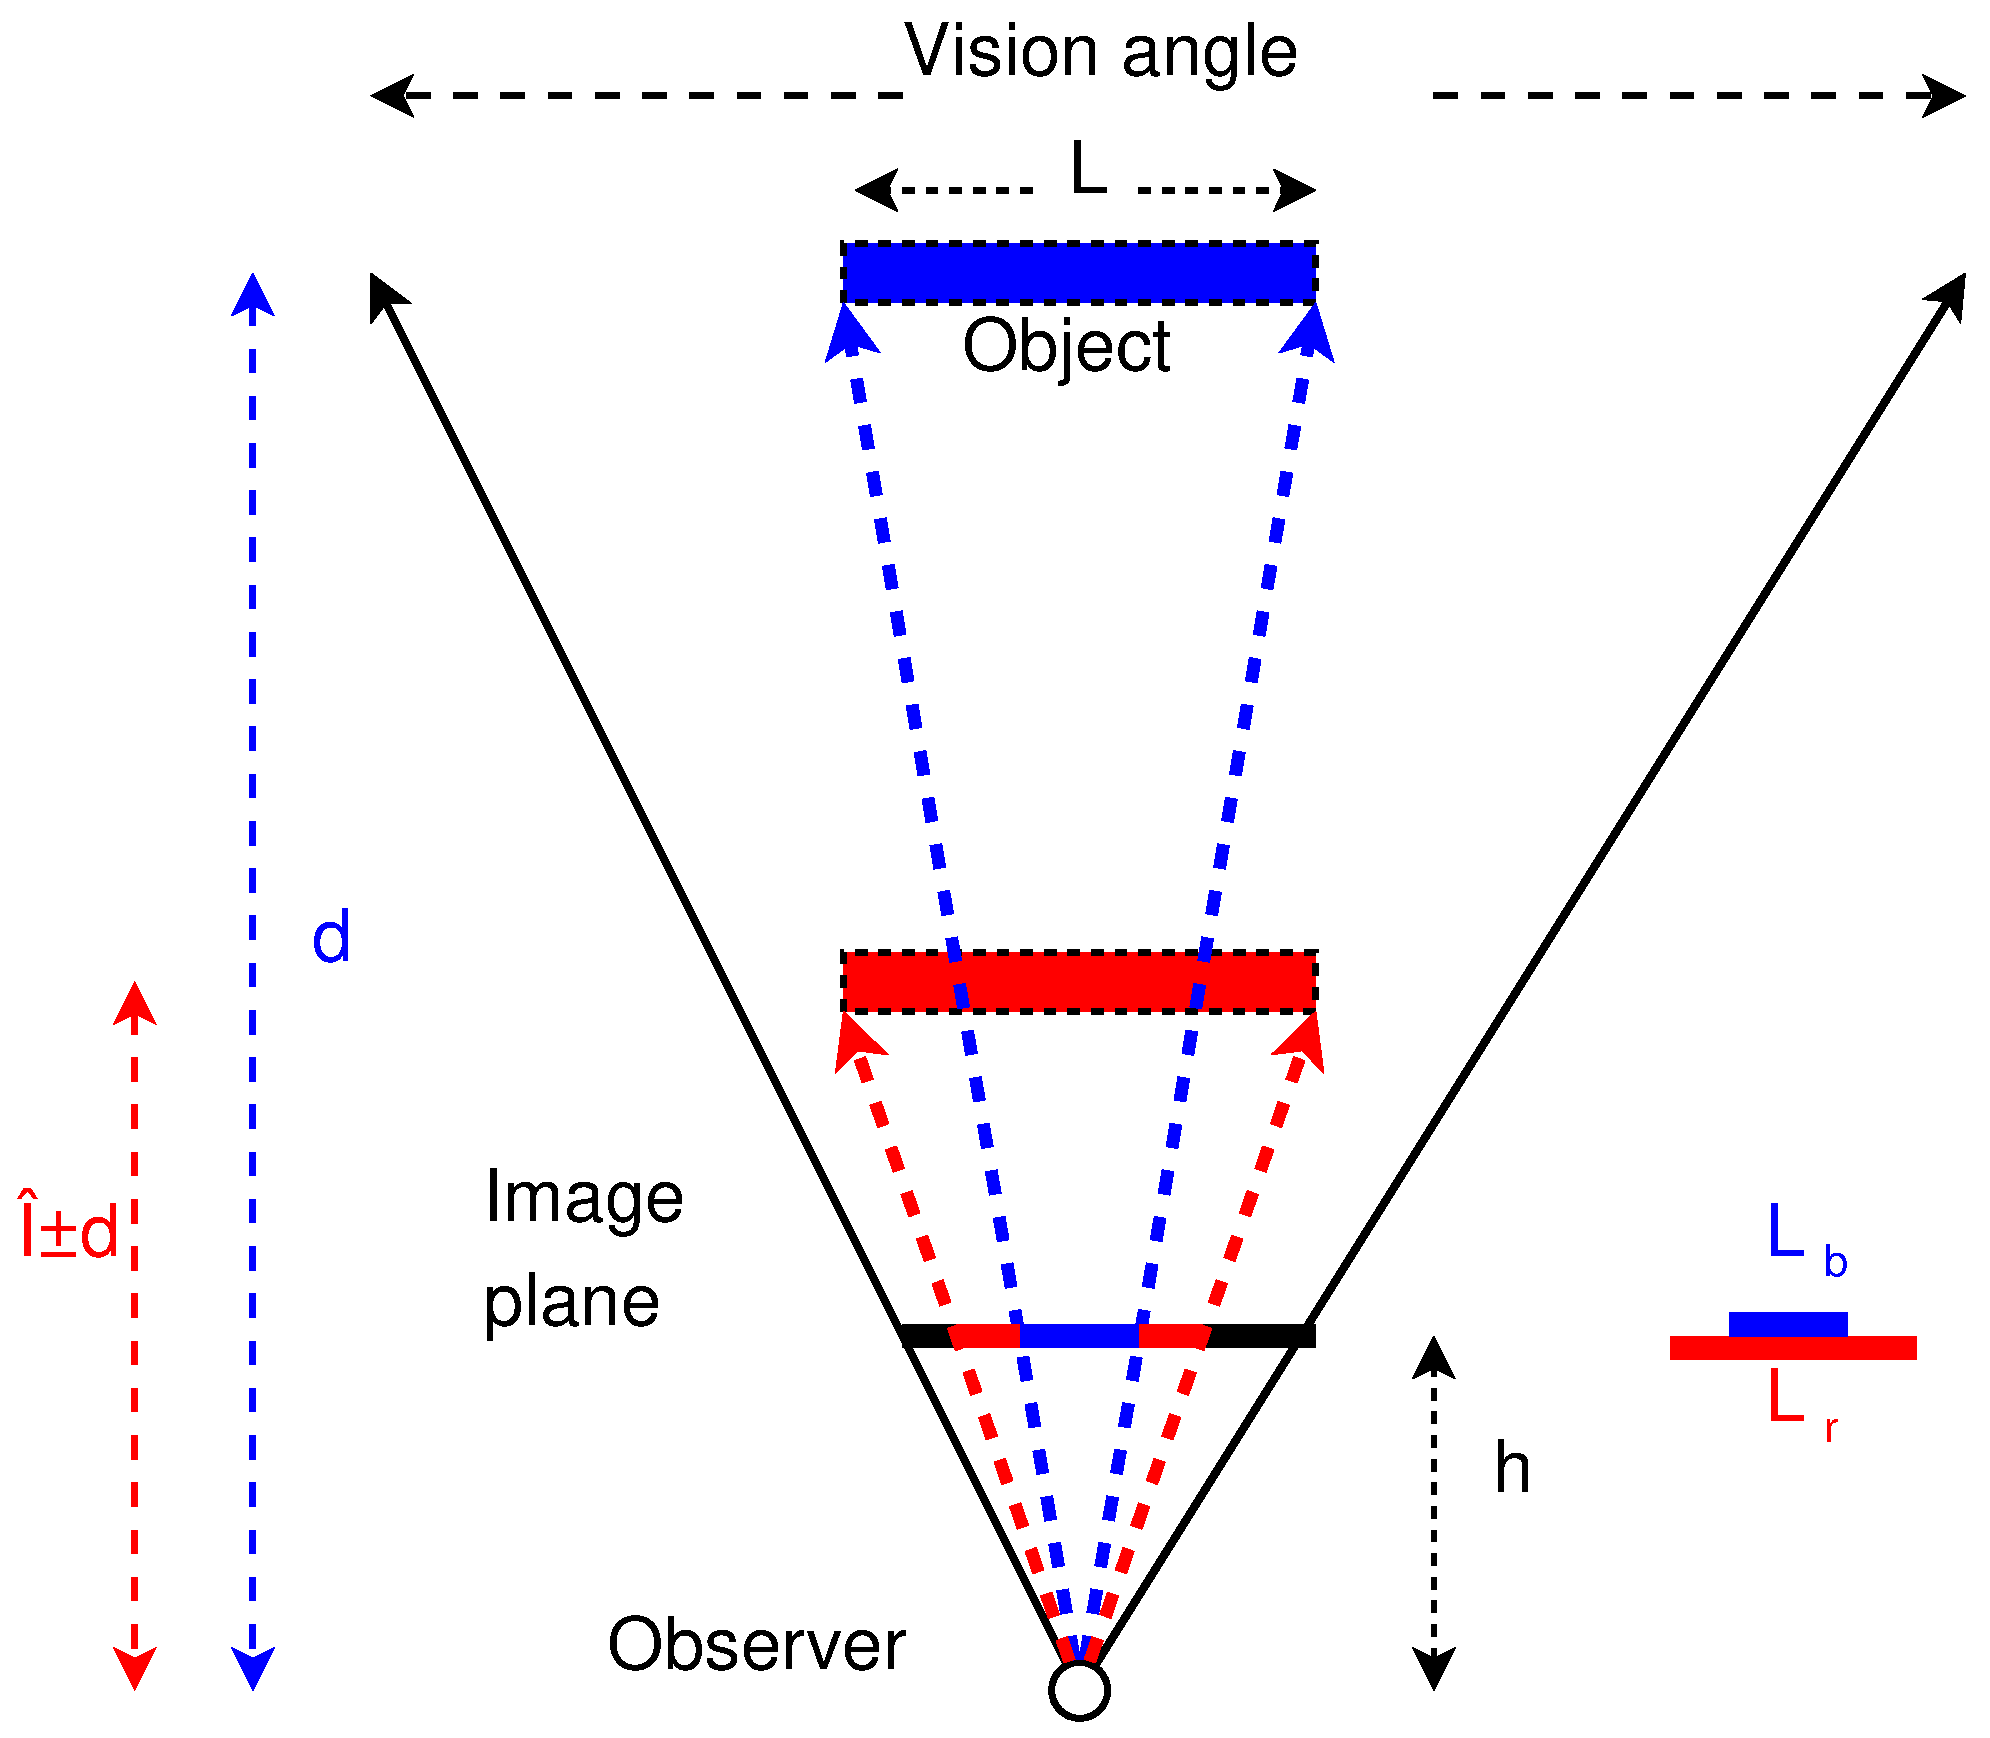
\includegraphics[width=.7\columnwidth]{images/Diagrama3.eps}
  \caption{The multi-scale tracking.}
  \label{fig:multiscale3d}
\end{figure}

Fig.\ref{fig:multiscale3d} shows the same target at two different distances $d$ and $\alpha d$, respectively, in blue and red.
The image plane is located at a distance $h$ of the observer.
The projections of objects, in blue and red, are labelled in the image as
$L_b$ and $L_r$, respectively. Making a simple inspection in the
formed triangles, we can see that $\frac{h}{d}=\frac{L_b}{L}$ and 
$\frac{h}{\alpha d}=\frac{L_r}{L}$, then $L_b/\alpha= L_r$. 
From the point of view of the observer, this implies that when a target 
was located at a distance $d$ at a time $t_0$,  and is moved to a distance $\alpha d$ at a time $t_1$, 
the width of the target in the image plane is altered by a factor of 1/$\alpha$, 
and consequently its area is altered by a factor of 1/$\alpha^2$.

The search criterion of objects uses different discrete values of $\alpha$, so that 
the algorithm tracks nearest objects with $\alpha<1$ and farthest objects  with $\alpha>1$.

%usa Multi-resolution match criteria e explica isso dos tamanhos

\subsubsection{DEPARTURE FACTOR - RELATIVE VELOCITY}
The departure factor is a dimensionless number related to the rate of approach 
or departure of a target to the observer. The factor
is determined in Eq. (\ref{eq:relarea}),

\begin{equation}\label{eq:relarea}
f_a \equiv \alpha^2 \equiv \frac{Area_r}{Area_f} 
\end{equation}

where $f_a$ and $\alpha$ are defined as factor area and departure factor, 
respectively; $Area_r$ is the ROI area and $Area_f$ 
is the analyzed region in the current image frame.

Thus, knowing $\alpha$, if we consider that the target in the $ROI$ was to a distance $d_{ROI}$,
then the target in the analysis region will be to a distance of $\alpha d_{ROI}$ (or $\sqrt{f_a} d_{ROI}$).
So that, each $i-th$ frame will have its own $\alpha_i$ value; where, $d_i=\alpha_i d_{ROI}$.

The departure factor, $\alpha_i$, has two interpretations: if the rate of departure increases quickly, 
this  means that the target is departing. If the factor decreases, the 
target is approaching.

The relative velocity is using a simple equation of kinematic in physics:
\begin{equation}
 v_i = \frac{\Delta s}{\Delta t}= \frac{s_i-s_{i-1}}{\Delta t}.
\end{equation}

where the vector $v_i$ represents the relative velocity in the i-th image frame, 
$s_i=(x_i,y_i,d_i)$ is the position of match in the i-th image frame
and $\Delta t$ is the sampling time between image frames.
Additionally, we call velocity of departure factor, $v^d_i$, 
the scalar number which represents the depth component
of the vector $v_i$.

The calculated  $v^d_i$ value is relative, for the simple reason that the distance (depth) between the 
camera (observer) and the target in the instance i-th will be referenced to $d_{ROI}$, 
given that the distance of the initial $ROI$ is established by definition to 1.
Finally, in all cases, the position $s_i$ is relative to the observer (a moving reference system).

\end{comment}

%%%%%%%%%%%%%%%%%%%%%%%%%%%%%%%portugues%%%%%%%%%%%%%%%%%%%%%%%%%%%%%%%%%%%%%%%%%%%%%%%


\subsubsection{Interpretação da busca em camadas - 3D}

Para compreender o método de busca em camadas é necessário analisar a projeção do objeto 
no plano da imagem para diferentes distancias do objeto com respeito ao observador, 
como mostrado na Figura \ref{fig:multiscale3d}.
\begin{figure}[H]
\centering
  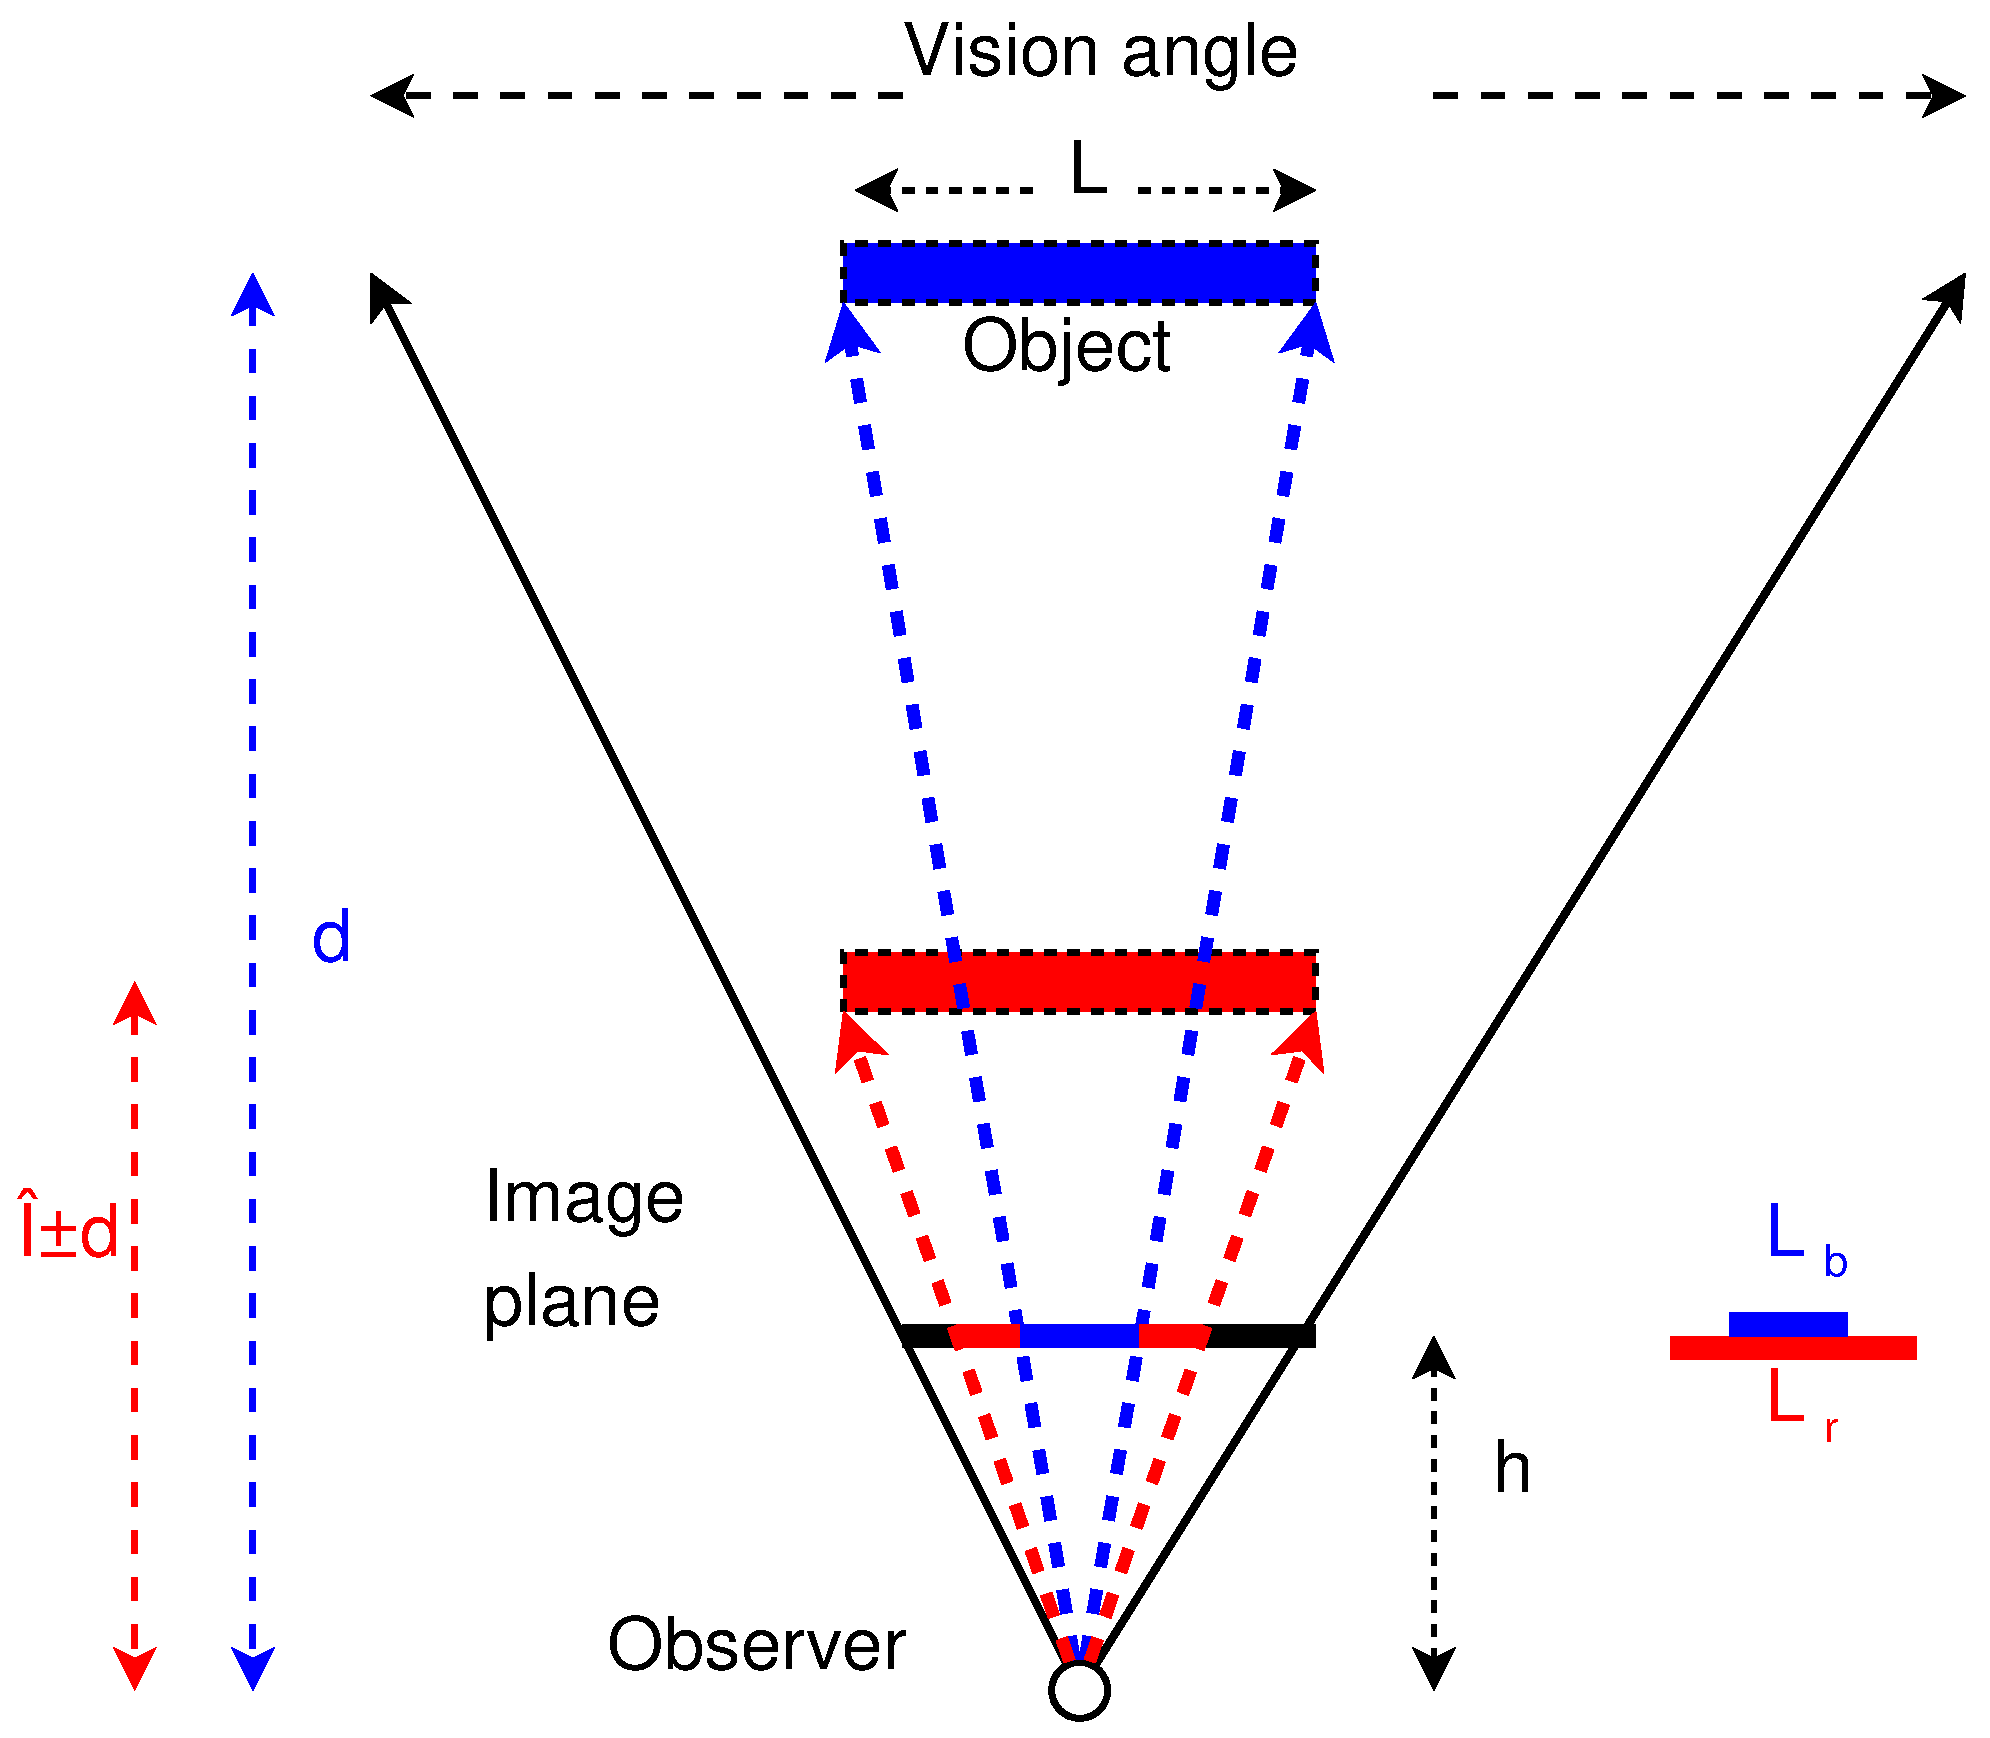
\includegraphics[width=.7\columnwidth]{images/Diagrama3.eps}
  \caption{ Acompanhamento do objeto em camadas.}
  \label{fig:multiscale3d}
\end{figure}
A Figura \ref{fig:multiscale3d} mostra o objeto de interesse a diferentes distanasias com respeito ao observador, 
$d$ e $\alpha d$, respectivamente em azul e vermelho, sendo que
o plano da imagem está localizada a uma distância $h$ do observador. As projeções dos objetos no plano da imagem
 são representados por $L_b$ e $L_r$, azul e vermelho respectivamente. 
 Analisando os triângulos formados pelas projeções dos objetos e o ponto de observação, 
 é possível notar que $\frac{h}{d}=\frac{L_b}{L}$ e $\frac{h}{\alpha d}=\frac{L_r}{L}$, logo 
$L_b/\alpha= L_r$. 
Assim, partindo do ponto de vista do observador, quando o objeto estava localizado a uma distância $d$ no tempo
$t_0$ e moveu-se para a distância $\alpha d$ no tempo $t_1$, o tamanho da projeção do objeto no plano da imagem 
foi alterado por um fator de 1/$\alpha$, e consequentemente, a área foi alterada por um fator 1/$\alpha^2$.

Conhecida a relação de $\alpha$ com a distancia entre o objeto e o observador; 
o critério de busca em $3D$, do objeto de interesse, usa um conjunto de valores 
discretos de $\alpha$ para determinar a localização, 
consequentemente se o objeto de interesse estiver localizado num ponto intermédio dos valores
de $\alpha$ selecionados, o algoritmo aproxima a posição do objeto 
usando o valor de $\alpha$ mais próximo; assim, são usados valores $\alpha<1$
para procurar objetos mais próximos que a posição $d_{ROI}$ e  $\alpha>1$ para mais distantes.



\subsubsection{Fator de aproximação - Velocidade Relativa}

O fator de aproximação é um número adimensional que relaciona a taxa de 
aproximação de um objeto em relação ao seu observador.
O fator é determinado pela Equação (\ref{eq:relarea}),

\begin{equation}\label{eq:relarea}
f_a \equiv \alpha^2 \equiv \frac{Area_r}{Area_f} 
\end{equation}

Onde $f_a$ e $\alpha$ são definidos como um fator de área e de aproximação,
respectivamente; $Area_r$ é a área do $ROI$ e $Area_f$ é a área da região analisada
do último frame.

Conhecendo $\alpha$, e se considerado que o objeto estava a uma distância $d_{ROI}$; então,
sua próxima distância será $\alpha d_{ROI}$ (ou $\sqrt{f_a} d_{ROI}$). Assim, cada $i-ésimo$ imagem
terá o seu próprio $\alpha_i$ valor, onde $d_i=\alpha_i d_{ROI}$.

O fator de aproximação, $\alpha_i$, tem dois significados: se o fator de aproximação cresce rapidamente 
significa que o objeto está se afastando e se o fator decresce o objeto está se aproximando.

A velocidade relativa é definida pela equação da cinemática em física:

\begin{equation}
 v_i = \frac{\Delta s}{\Delta t}= \frac{s_i-s_{i-1}}{\Delta t}.
\end{equation}

Onde o vetor $v_i$ representa a velocidade relativa à $i-ésimo$ imagem, $s_i=(x_i,y_i,d_i)$ é a posição que
foi definida pela busca na $i-ésimo$ imagem e $\Delta t$ é o intervalo de tempo entre a análise das duas imagens.
Adicionalmente, o fator da velocidade de aproximação, $v^d_i$, é o número escalar o qual representa a componente
responsável pela profundidade no vetor $v_i$.

O valor $v^d_i$ calculado é relativo, pelo simples motivo de que a distância (profundidade) entre a câmara 
(observador) e o alvo no instante $i-ésimo$ será referenciada para $d_{ROI}$; assim a distância do $ROI$ 
inicial é estabelecida por definição para $d_{ROI}=1$. Finalmente, em todos os casos, a posição é 
relativa ao observador (um sistema de referência móvel).

